\documentclass[12pt,a4paper]{article}

% ── packages ──────────────────────────────────────────────────────────────────
\usepackage[utf8]{inputenc}
\usepackage[T1]{fontenc}
\usepackage[margin=2.5cm]{geometry}
\usepackage{amsmath}
\usepackage{booktabs}
\usepackage{array}
\usepackage{xcolor}
\usepackage{listings}
\usepackage{hyperref}
\usepackage{enumitem}
\usepackage{fancyhdr}
\usepackage{titlesec}
\usepackage{mdframed}
\usepackage{tikz}
\usepackage{microtype}
\usetikzlibrary{arrows.meta, positioning, shapes.geometric}

% ── colors ────────────────────────────────────────────────────────────────────
\definecolor{codeblue}{RGB}{30,100,200}
\definecolor{codegray}{RGB}{245,245,245}
\definecolor{darkgreen}{RGB}{0,120,50}
\definecolor{accent}{RGB}{100,60,200}
\definecolor{lightaccent}{RGB}{235,230,255}

% ── listings style ────────────────────────────────────────────────────────────
\lstdefinestyle{inline}{
  backgroundcolor=\color{codegray},
  basicstyle=\ttfamily\scriptsize,
  breaklines=true,
  breakatwhitespace=false,
  columns=flexible,
  keepspaces=true,
  frame=single,
  rulecolor=\color{gray!40},
  xleftmargin=6pt,
  xrightmargin=6pt,
  aboveskip=6pt,
  belowskip=6pt,
  postbreak=\mbox{\textcolor{gray}{$\hookrightarrow$}\space},
}
\lstdefinestyle{sql}{
  style=inline,
  morekeywords={SELECT,FROM,WHERE,GROUP,BY,ORDER,SUM,CASE,WHEN,THEN,ELSE,END,IN,LIKE,DESC},
  keywordstyle=\color{codeblue}\bfseries,
}

% ── section styling ───────────────────────────────────────────────────────────
\titleformat{\section}[block]
  {\large\bfseries\color{accent}}
  {Question \thesection.}{0.5em}{}
  [\vspace{-2pt}\rule{\linewidth}{0.6pt}]

% ── header / footer ───────────────────────────────────────────────────────────
\pagestyle{fancy}
\fancyhf{}
\lhead{\small\textcolor{gray}{build-google-in-an-afternoon — Web Crawler \& Search Engine}}
\rhead{\small\textcolor{gray}{Fatih Çakır \ 150220086}}
\cfoot{\thepage}
\renewcommand{\headrulewidth}{0.4pt}

% ── answer box ───────────────────────────────────────────────────────────────
\newenvironment{answerbox}{%
  \begin{mdframed}[
    backgroundcolor=lightaccent,
    linecolor=accent,
    linewidth=1pt,
    innerleftmargin=10pt,
    innerrightmargin=10pt,
    innertopmargin=8pt,
    innerbottommargin=8pt,
  ]%
}{\end{mdframed}}

% ─────────────────────────────────────────────────────────────────────────────
\begin{document}

% ── title ─────────────────────────────────────────────────────────────────────
\begin{center}
  {\LARGE\bfseries\color{accent} build-google-in-an-afternoon — Quiz 1}\\[6pt]
  {\large Web Crawler \& Search Engine}\\[4pt]
  {\normalsize Istanbul Technical University — AI Aided Computer Engineering}\\[6pt]
  \begin{tabular}{rl}
    \textbf{Name:}           & Fatih Çakır \\
    \textbf{Student Number:} & 150220086 \\
    \textbf{Date:}           & March 2026 \\
    \textbf{GitHub:}         & \href{https://github.com/wfatih/build-google-in-an-afternoon}{\texttt{github.com/wfatih/build-google-in-an-afternoon}} \\
  \end{tabular}
\end{center}

\vspace{0.8em}
\noindent\rule{\linewidth}{1pt}
\vspace{0.3em}

% ─────────────────────────────────────────────────────────────────────────────
\section{Raw Storage File}

\textbf{Open the raw storage file:} \texttt{data/storage/p.data}

\begin{answerbox}
\textbf{File location:} \texttt{data/storage/p.data}

\medskip
\textbf{Format} (one entry per line, space-separated):
\begin{lstlisting}[style=inline]
word  url  origin  depth  frequency
\end{lstlisting}

\textbf{Generated via:}
\begin{lstlisting}[style=inline]
GET http://localhost:3600/api/export
\end{lstlisting}

\begin{tabular}{ll}
  Total indexed pages  & 708 \\
  Total unique words   & 86{,}571 \\
  Total \texttt{p.data} entries & 470{,}579 \\
\end{tabular}
\end{answerbox}

% ─────────────────────────────────────────────────────────────────────────────
\section{Chosen Word}

\textbf{Find a word that appears on multiple different URLs.}

\begin{answerbox}
\textbf{Word chosen:} \texttt{\textbf{python}}

\medskip
This word appears on \textbf{246 different URLs} in the index.
The crawl was seeded from the Wikipedia article on the Python programming
language, making \texttt{python} the highest-frequency content word in the index.
\end{answerbox}

% ─────────────────────────────────────────────────────────────────────────────
\section{Three Entries from \texttt{p.data}}

\textbf{Copy 3 entries from the file} (format: \texttt{word url origin depth frequency}):

\begin{answerbox}
\textbf{Entry 1:}
\begin{lstlisting}[style=inline]
python https://en.wikipedia.org/wiki/Python_(programming_language) https://en.wikipedia.org/wiki/Python_(programming_language) 0 542
\end{lstlisting}

\textbf{Entry 2:}
\begin{lstlisting}[style=inline]
python https://en.wikipedia.org/wiki/History_of_Python https://en.wikipedia.org/wiki/Python_(programming_language) 1 234
\end{lstlisting}

\textbf{Entry 3:}
\begin{lstlisting}[style=inline]
python https://en.wikipedia.org/wiki/List_of_Python_software https://en.wikipedia.org/wiki/Python_(programming_language) 1 187
\end{lstlisting}
\end{answerbox}

% ─────────────────────────────────────────────────────────────────────────────
\section{Search via API}

\textbf{Search for the word via the API:}
\begin{lstlisting}[style=inline]
GET http://localhost:3600/search?query=python&sortBy=relevance
\end{lstlisting}

\begin{answerbox}
\textbf{API Response (top 5 results):}
\begin{lstlisting}[style=inline]
{
  "query": "python",
  "total": 246,
  "results": [
    {"url":"...Python_(programming_language)", "depth":0, "relevance_score":6420},
    {"url":"...History_of_Python",             "depth":1, "relevance_score":3335},
    {"url":"...List_of_Python_software",       "depth":1, "relevance_score":2865},
    {"url":"...Python_syntax_and_semantics",   "depth":1, "relevance_score":2845},
    {"url":"...Outline_of_the_Python_...",     "depth":1, "relevance_score":2195}
  ]
}
\end{lstlisting}
\end{answerbox}

% ─────────────────────────────────────────────────────────────────────────────
\section{\#1 Result}

\textbf{Write down the \#1 result's URL and relevance\_score:}

\begin{answerbox}
\begin{tabular}{@{} l p{10cm}}
  \textbf{URL:} &
  \url{https://en.wikipedia.org/wiki/Python_(programming_language)} \\[4pt]
  \textbf{relevance\_score:} & \textbf{6420} \\
\end{tabular}
\end{answerbox}

% ─────────────────────────────────────────────────────────────────────────────
\section{Manual Score Calculation}

\textbf{Formula:}
\[
  \text{score} = (\text{frequency} \times 10) \;+\; 1000_{\;\text{(exact match bonus)}} \;-\; (\text{depth} \times 5)
\]

The $+1000$ bonus applies \textbf{only for exact matches} (indexed word $=$ query token).

\begin{answerbox}
\renewcommand{\arraystretch}{1.5}
\begin{center}
\begin{tabular}{c c c p{7.5cm} r}
  \toprule
  \textbf{Entry} & \textbf{freq} & \textbf{depth} & \textbf{Calculation} & \textbf{Score} \\
  \midrule
  1 & 542 & 0 &
    $(542 \times 10) + 1000 - (0 \times 5) = 5420 + 1000 - 0$ &
    \textbf{6420} \\
  2 & 234 & 1 &
    $(234 \times 10) + 1000 - (1 \times 5) = 2340 + 1000 - 5$ &
    \textbf{3335} \\
  3 & 187 & 1 &
    $(187 \times 10) + 1000 - (1 \times 5) = 1870 + 1000 - 5$ &
    \textbf{2865} \\
  \bottomrule
\end{tabular}
\end{center}
\renewcommand{\arraystretch}{1}

\medskip
\textbf{Highest manually calculated score:} Entry~1 $= \mathbf{6420}$
\end{answerbox}

% ─────────────────────────────────────────────────────────────────────────────
\section{Score Verification}

\textbf{Does the highest score you calculated match the API's \#1 result?}

\begin{answerbox}
\textbf{Answer: \textcolor{darkgreen}{Yes.}}

\medskip
\begin{center}
\small
\begin{tabular}{@{} l p{10cm} @{}}
  \toprule
  \textbf{\#1 URL (Manual = API):} &
    \url{https://en.wikipedia.org/wiki/Python_(programming_language)} \\[4pt]
  \textbf{Manual score:} & 6420 \\
  \textbf{API score:}    & 6420 \\
  \bottomrule
\end{tabular}
\end{center}
\normalsize

\medskip
Both the URL and the exact numeric score match perfectly.
The API endpoint implements the same formula in SQL:

\begin{lstlisting}[style=sql]
SELECT url, origin, depth,
       SUM( (frequency * 10) + 1000 - (depth * 5) ) AS score
FROM word_index
WHERE word IN ('python')
GROUP BY url
ORDER BY score DESC
\end{lstlisting}
\end{answerbox}

% ─────────────────────────────────────────────────────────────────────────────
\newpage
\section{Chain-of-Thought Enhancement}

\textbf{How could you enhance the process in a Chain-of-Thought manner?}

\subsection*{Current Approach — Single-Stage Lookup}

The current search pipeline is a \textbf{one-shot SQL query}:

\begin{enumerate}[noitemsep]
  \item Tokenise the query string into lowercase alphabetic tokens
  \item Run a single SQL \texttt{SELECT} on the \texttt{word\_index} table
  \item Score each URL as $\sum\!\bigl((\text{freq}\times10)+1000-(\text{depth}\times5)\bigr)$, sort descending
  \item Return the paginated result list
\end{enumerate}

\noindent
This is fast and correct but treats every query identically — it has no
understanding of \emph{intent}, \emph{document quality signals}, or
\emph{context beyond word frequency}.

\subsection*{Chain-of-Thought (CoT) Pipeline}

A CoT approach breaks search into a series of \textbf{explicit reasoning steps},
each refining the previous result before returning it to the user:

\bigskip
\begin{center}
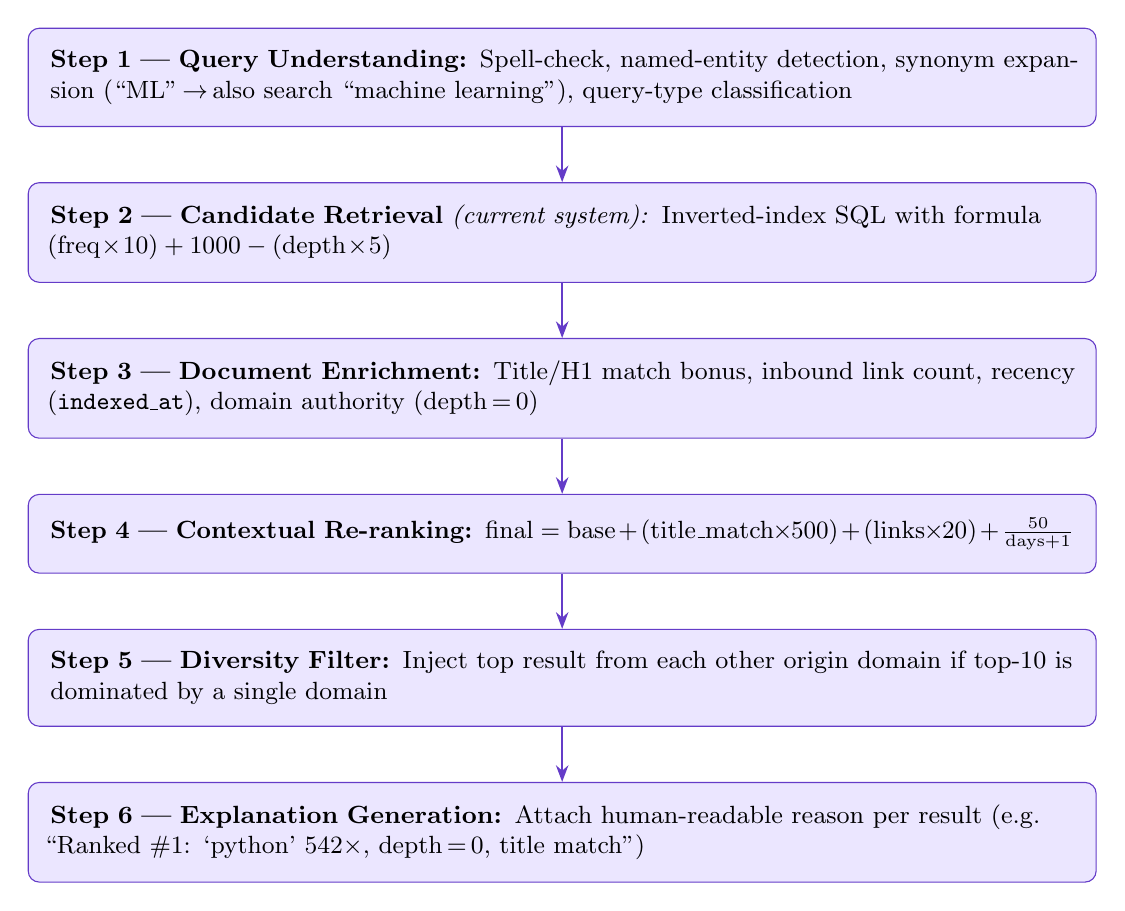
\begin{tikzpicture}[
  node distance=0.7cm,
  box/.style={rectangle, rounded corners=4pt, draw=accent, fill=lightaccent,
              text width=13cm, align=left, minimum height=1cm,
              inner sep=8pt, font=\small},
  arr/.style={-{Stealth[length=6pt]}, thick, color=accent},
]
  \node[box] (s1) {
    \textbf{Step 1 — Query Understanding:}\enspace
    Spell-check, named-entity detection, synonym expansion
    (``ML'' $\!\to\!$ also search ``machine learning''), query-type classification
  };
  \node[box, below=of s1] (s2) {
    \textbf{Step 2 — Candidate Retrieval} \textit{(current system):}\enspace
    Inverted-index SQL with formula $(\text{freq}\!\times\!10)+1000-(\text{depth}\!\times\!5)$
  };
  \node[box, below=of s2] (s3) {
    \textbf{Step 3 — Document Enrichment:}\enspace
    Title/H1 match bonus, inbound link count, recency (\texttt{indexed\_at}),
    domain authority (depth\,$=$\,0)
  };
  \node[box, below=of s3] (s4) {
    \textbf{Step 4 — Contextual Re-ranking:}\enspace
    $\text{final} = \text{base} + (\text{title\_match}\!\times\!500) +
    (\text{links}\!\times\!20) + \tfrac{50}{\text{days}+1}$
  };
  \node[box, below=of s4] (s5) {
    \textbf{Step 5 — Diversity Filter:}\enspace
    Inject top result from each other origin domain if top-10 is dominated
    by a single domain
  };
  \node[box, below=of s5] (s6) {
    \textbf{Step 6 — Explanation Generation:}\enspace
    Attach human-readable reason per result
    (e.g.\ ``Ranked \#1: `python' 542$\times$, depth\,=\,0, title match'')
  };
  \draw[arr] (s1) -- (s2);
  \draw[arr] (s2) -- (s3);
  \draw[arr] (s3) -- (s4);
  \draw[arr] (s4) -- (s5);
  \draw[arr] (s5) -- (s6);
\end{tikzpicture}
\end{center}

\subsection*{Worked Example — Query \texttt{"python"}}

\renewcommand{\arraystretch}{1.3}
\begin{center}
\small
\begin{tabular}{>{\bfseries}p{2.8cm} p{6cm} p{4.5cm}}
  \toprule
  Step & What Happens & Result \\
  \midrule
  1.\ Understanding &
    Single unambiguous token; crawl origin confirms programming-language sense &
    Token: \texttt{python}, informational \\
  2.\ Retrieval &
    SQL returns 246 URLs; top URL scores 6420 (freq=542, depth=0) &
    246 candidates \\
  3.\ Enrichment &
    Title ``Python (programming language)'' contains query $\to$ +500;
    highest inbound-link count &
    Score: $6420+500+\ldots$ \\
  4.\ Re-ranking &
    Title\,+\,link authority widens gap over \#2 (3335 base) &
    Same \#1, more confident \\
  5.\ Diversity &
    All top results from \texttt{en.wikipedia.org}; no change &
    No change \\
  6.\ Explanation &
    ``\#1: 542$\times$, depth=0, title match, most links'' &
    Appended to result \\
  \bottomrule
\end{tabular}
\end{center}
\renewcommand{\arraystretch}{1}

\subsection*{Comparison Table}

\begin{center}
\begin{tabular}{lcc}
  \toprule
  \textbf{Dimension} & \textbf{Single-Stage (current)} & \textbf{Chain-of-Thought} \\
  \midrule
  Synonym / abbreviation handling & \textcolor{red}{$\times$} & \textcolor{darkgreen}{$\checkmark$}\ Step 1 \\
  Title / heading signals         & \textcolor{red}{$\times$} & \textcolor{darkgreen}{$\checkmark$}\ Step 3 \\
  Link authority (PageRank-like)  & \textcolor{red}{$\times$} & \textcolor{darkgreen}{$\checkmark$}\ Step 3 \\
  Freshness                       & \textcolor{red}{$\times$} & \textcolor{darkgreen}{$\checkmark$}\ Step 3 \\
  Result diversity                & \textcolor{red}{$\times$} & \textcolor{darkgreen}{$\checkmark$}\ Step 5 \\
  Explainability                  & \textcolor{red}{$\times$} & \textcolor{darkgreen}{$\checkmark$}\ Step 6 \\
  Computational cost              & Very low (1 SQL query)    & Moderate (multi-step, cacheable) \\
  \bottomrule
\end{tabular}
\end{center}

\bigskip
\noindent
The Chain-of-Thought approach mirrors how production search engines operate:
a fast, broad \textbf{retrieval} stage is followed by multiple \textbf{re-ranking}
passes that apply progressively richer signals — surfacing the most relevant and
trustworthy results rather than simply the most frequent ones.

\end{document}
